\chapter{Background}

While the Earth's atmosphere is thick enough to cause more objects that pass through it, some can and will make it through. Theses are the objects of most importance to those observing fireballs, meteoroids, and meteors. This chapter will provide a more in-depth look at what classifies an object as a fireball, how these fireballs are detected both by other systems around the world and the D6, and discuss why and how the detected images are analyzed.

\section{What Exactly are Fireballs?}

The first thing to take into account when discussing meteoroids, meteors, fireballs, and even asteroids, is that they are all different and shouldn't be used interchangeably. 
An asteroid is not a meteoroid, a meteoroid is not a meteor, a fireball is a classification of meteor, and a bolide is a fireball that blows up in the atmosphere. 
This section will go into a little more detail regarding the various definitions of these space objects, 

Asteroids are meteoroids that are greater than 1 meter wide, as can be seen in figure 3, they tend to be concentrated outside of the Earth's orbit, as can be seen in the third figure.
As can be seen from this concentration, and from what has been determined by the scientific community, large asteroid impacts tend to occur rather rarely, with "an automobile sized asteroid" entering the atmosphere about once a year \cite{atkinson_2018}. 
Meteoroids however, are the little siblings of asteroids, and are of just as much interest.

\begin{figure}
    \centering
    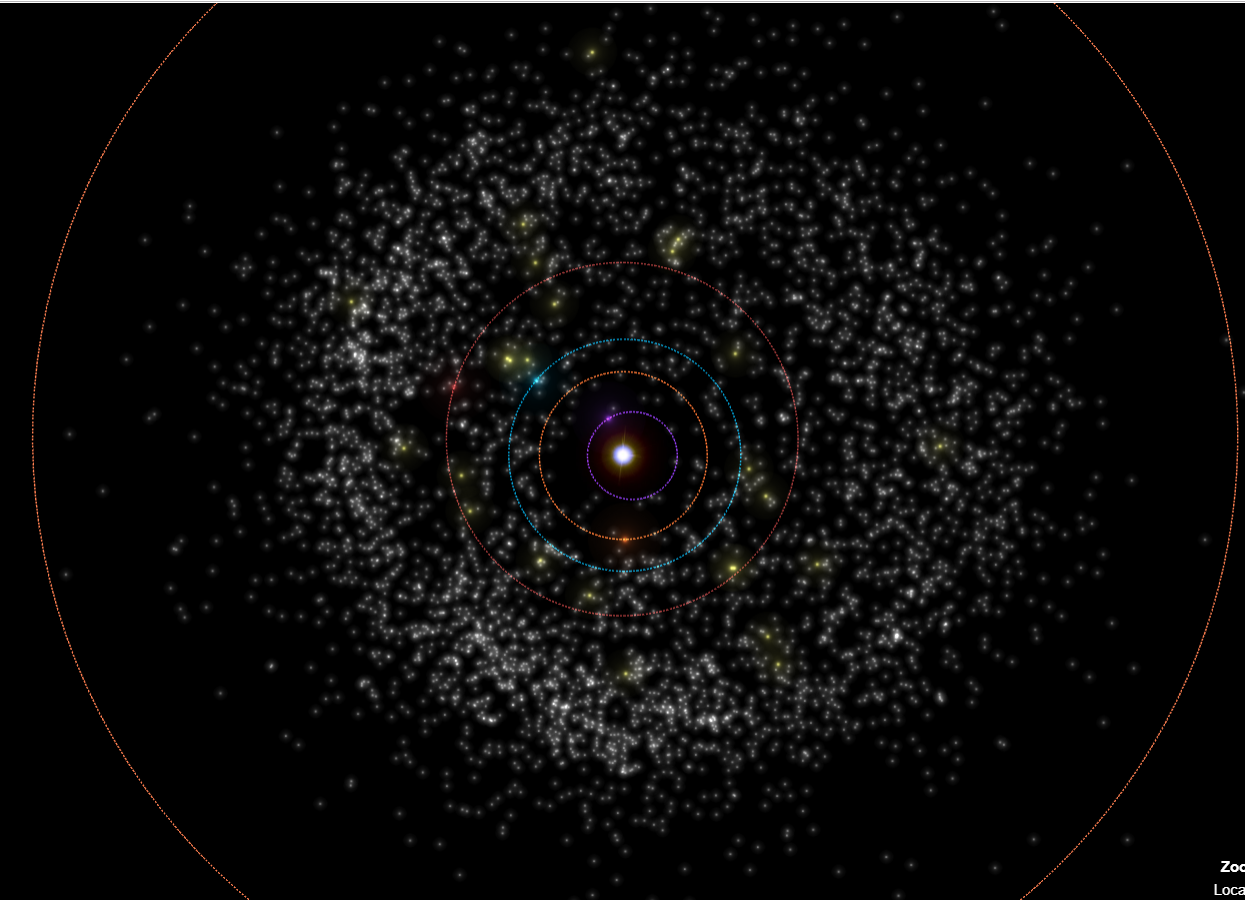
\includegraphics[width=12cm]{Solar-System-Asteroids.png}
    \centering
    \caption{Image of asteroid plots in our Solar System, courtesy of Asterank, as can be seen the asteroids mainly orbit outside the orbit of the Earth, though some do merge in and out of the Earth's orbit.}
    \label{Figure 3}
\end{figure}

Meteoroids are any bits and bobs of cosmic space debris that are up to 1 meter in width, from dust to small pieces of rock blasted off from asteroid collisions. 
The only true difference between an asteroid and a meteoroid is that one is large, while one is usually much smaller, with the meteroid being frequently only millimeters in size \cite{atkinson_2018}. 
When both asteroids and meteoroids hit the atmosphere and begin leaving a streak of fire across the sky, they are then referred to as meteors. 
While meteors are harmless most of the time, they can turn into bolides, also known as fireballs \cite{atkinson_2018}. 

Fireballs, or bolides, will be the main focus of the project, as they are what are being observed for by the D6 and the other detection systems that the D6 will be compared to when determining it's effectiveness. 
Fireballs are meteors that have especially bright trails, and tend to either burn out in the atmosphere, explode, or leave behind a meteorite like the one that occurred over Spain, Portugal, and France, with a meteorite being left behind in northern Palencia \cite{Villabeto}. 
In the next segment a more in depth look will be taken at the different methods used to detect the fireballs, as well as some of positives and negatives for each of these detection methods.

\section{Methods of Detection}

One of the major detection networks is called CAMS, or, Cameras for Allsky Meteor Surveillance. 
The goal of this NASA funded project is to validating unconfirmed meteor showers by measuring velocity vectors and times of arrival and from that information, determining if various detected meteoroids and fireballs originated from the same group passing through the Earth's orbit \cite{jenniskens}. 
The stations for the detection network contain a box within which twenty Watec 902 H2 Ultimate video cameras, an interesting feature of this camera setup is that it comes with a sun shade, which can be used to protect the setup from bad weather. 
The sun shade also helps protect the sensitive cameras from direct sunlight during daytime hours \cite{jenniskens}. 
An important feature of this setup to note is that the camera also has a battery mounted nearby to support it, as well as the linux surveillance servers required to process and store the data from each of the cameras.
As can be seen in Figures 4 and 5, the total setup is fairly bulky, although the use of an array of cameras for comparison will allow for fairly good detail in any capture images, as well as the capability to determine the velocity of a fireball as it moves across the array.

\begin{figure}
    \centering
    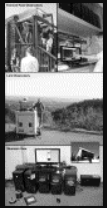
\includegraphics[scale=1.5]{CAMS-Server-Setup.png}
    \caption{Image of the Server setup for the CAMS network, from \cite{jenniskens}}
    \label{Figure 4}
\end{figure}

\begin{figure}
    \centering
    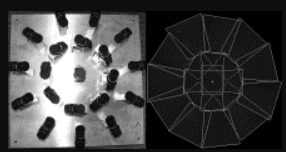
\includegraphics[scale=1.5]{CAMS-Camera-Setup.png}
    \caption{Image of the Camera setup for the CAMS network, from \cite{jenniskens}}
    \label{Figure 5}
\end{figure}

Another system is the SPMN, or Spanish Meteor Network, where instead of having an array of cameras at each station, each video station uses a high sensitivity CCTV camera, with there being 11 of the high sensitivity cameras in total \cite{SPMN}. 
An interesting feature of this system is that each camera will have an Aspherical fast lens that will have a focal length ranging from 2.6 mm, which is a fish-eye lens, to 12mm and a focal ratio between 1.2 and 0.8 for the imaging reflective lens. 
These different lens types will allow various areas of the sky to be covered by each and every camera, and images across the entire field of view can be captured \cite{SPMN}.
As with the CAMS system, the SPMN can also determine the velocity of a fireball or bolide by capturing the meteor and tracking it across the sky using a video time inserter that has a GPS device. 
This allows for an accuracy of $10^-1$ seconds while tracking the meteor along its path across the night sky \cite{SPMN}.

The third detection system that will be discussed in this paper is of course, the Willamette University D6 AllSky Camera. 
The D6 was created in 2016 to, like the previous two detection systems, detect fireballs streaking across the night sky.
The idea behind the D6 is to create a system that is cheaper and easier to move than systems such as CAMS or SPMN. 
To do this, a Raspberry Pie was used as the computational support for the camera system, instead of the more traditional number crunching towes used in CAMS of SPMN \cite{McSwain}.
The D6 itself looks a bit like a short traffic bollard, with a plastic dome covering the Watec902H2 CCD camera, and a PVC pipe acting as the housing for all the internal units of the D6.
Inside, besides the camera and Raspberry Pi, is a thermostat with accompanying heater to ensure that moisture doesn't accumulate inside the housing, as well as a digitizer to convert the film taken by the camera from analog to digital so that it can be analyzed. A image of the camera from PJ Gibsons thesis can be found in figure 6.

\begin{figure}
    \centering
    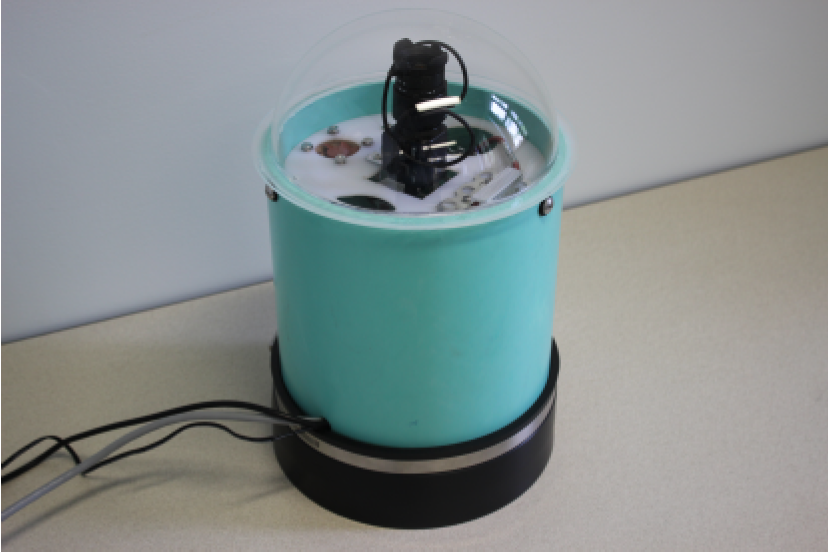
\includegraphics[width=10cm]{D6-Camera.png}
    \caption{Image of the Camera setup for the CAMS network, from \cite{Gibson}}
    \label{Figure 6}
\end{figure}

When the camera detects a fireball passing through its field of view, it takes footage of said event, and then the footage in converted by the digitizer into a form suitable for the Raspberry Pi to collect and store, with the data being accessed by a laptop at a later date for future analysis using code that will be discussed in the next section.

\section{Previous Work Done on the Project}

How it's analyzed, discuss Luke's luminosity code, PJ's work with observational area, how we want to measure the flux based off observational energy.